\documentclass[]{book}
\usepackage{lmodern}
\usepackage{amssymb,amsmath}
\usepackage{ifxetex,ifluatex}
\usepackage{fixltx2e} % provides \textsubscript
\ifnum 0\ifxetex 1\fi\ifluatex 1\fi=0 % if pdftex
  \usepackage[T1]{fontenc}
  \usepackage[utf8]{inputenc}
\else % if luatex or xelatex
  \ifxetex
    \usepackage{mathspec}
  \else
    \usepackage{fontspec}
  \fi
  \defaultfontfeatures{Ligatures=TeX,Scale=MatchLowercase}
\fi
% use upquote if available, for straight quotes in verbatim environments
\IfFileExists{upquote.sty}{\usepackage{upquote}}{}
% use microtype if available
\IfFileExists{microtype.sty}{%
\usepackage[]{microtype}
\UseMicrotypeSet[protrusion]{basicmath} % disable protrusion for tt fonts
}{}
\PassOptionsToPackage{hyphens}{url} % url is loaded by hyperref
\usepackage[unicode=true]{hyperref}
\hypersetup{
            pdftitle={Particle Based Samplers for MCMC},
            pdfauthor={Jon-Paul Cavallaro},
            pdfborder={0 0 0},
            breaklinks=true}
\urlstyle{same}  % don't use monospace font for urls
\usepackage{natbib}
\bibliographystyle{apalike}
\usepackage{color}
\usepackage{fancyvrb}
\newcommand{\VerbBar}{|}
\newcommand{\VERB}{\Verb[commandchars=\\\{\}]}
\DefineVerbatimEnvironment{Highlighting}{Verbatim}{commandchars=\\\{\}}
% Add ',fontsize=\small' for more characters per line
\usepackage{framed}
\definecolor{shadecolor}{RGB}{248,248,248}
\newenvironment{Shaded}{\begin{snugshade}}{\end{snugshade}}
\newcommand{\KeywordTok}[1]{\textcolor[rgb]{0.13,0.29,0.53}{\textbf{#1}}}
\newcommand{\DataTypeTok}[1]{\textcolor[rgb]{0.13,0.29,0.53}{#1}}
\newcommand{\DecValTok}[1]{\textcolor[rgb]{0.00,0.00,0.81}{#1}}
\newcommand{\BaseNTok}[1]{\textcolor[rgb]{0.00,0.00,0.81}{#1}}
\newcommand{\FloatTok}[1]{\textcolor[rgb]{0.00,0.00,0.81}{#1}}
\newcommand{\ConstantTok}[1]{\textcolor[rgb]{0.00,0.00,0.00}{#1}}
\newcommand{\CharTok}[1]{\textcolor[rgb]{0.31,0.60,0.02}{#1}}
\newcommand{\SpecialCharTok}[1]{\textcolor[rgb]{0.00,0.00,0.00}{#1}}
\newcommand{\StringTok}[1]{\textcolor[rgb]{0.31,0.60,0.02}{#1}}
\newcommand{\VerbatimStringTok}[1]{\textcolor[rgb]{0.31,0.60,0.02}{#1}}
\newcommand{\SpecialStringTok}[1]{\textcolor[rgb]{0.31,0.60,0.02}{#1}}
\newcommand{\ImportTok}[1]{#1}
\newcommand{\CommentTok}[1]{\textcolor[rgb]{0.56,0.35,0.01}{\textit{#1}}}
\newcommand{\DocumentationTok}[1]{\textcolor[rgb]{0.56,0.35,0.01}{\textbf{\textit{#1}}}}
\newcommand{\AnnotationTok}[1]{\textcolor[rgb]{0.56,0.35,0.01}{\textbf{\textit{#1}}}}
\newcommand{\CommentVarTok}[1]{\textcolor[rgb]{0.56,0.35,0.01}{\textbf{\textit{#1}}}}
\newcommand{\OtherTok}[1]{\textcolor[rgb]{0.56,0.35,0.01}{#1}}
\newcommand{\FunctionTok}[1]{\textcolor[rgb]{0.00,0.00,0.00}{#1}}
\newcommand{\VariableTok}[1]{\textcolor[rgb]{0.00,0.00,0.00}{#1}}
\newcommand{\ControlFlowTok}[1]{\textcolor[rgb]{0.13,0.29,0.53}{\textbf{#1}}}
\newcommand{\OperatorTok}[1]{\textcolor[rgb]{0.81,0.36,0.00}{\textbf{#1}}}
\newcommand{\BuiltInTok}[1]{#1}
\newcommand{\ExtensionTok}[1]{#1}
\newcommand{\PreprocessorTok}[1]{\textcolor[rgb]{0.56,0.35,0.01}{\textit{#1}}}
\newcommand{\AttributeTok}[1]{\textcolor[rgb]{0.77,0.63,0.00}{#1}}
\newcommand{\RegionMarkerTok}[1]{#1}
\newcommand{\InformationTok}[1]{\textcolor[rgb]{0.56,0.35,0.01}{\textbf{\textit{#1}}}}
\newcommand{\WarningTok}[1]{\textcolor[rgb]{0.56,0.35,0.01}{\textbf{\textit{#1}}}}
\newcommand{\AlertTok}[1]{\textcolor[rgb]{0.94,0.16,0.16}{#1}}
\newcommand{\ErrorTok}[1]{\textcolor[rgb]{0.64,0.00,0.00}{\textbf{#1}}}
\newcommand{\NormalTok}[1]{#1}
\usepackage{longtable,booktabs}
% Fix footnotes in tables (requires footnote package)
\IfFileExists{footnote.sty}{\usepackage{footnote}\makesavenoteenv{long table}}{}
\usepackage{graphicx,grffile}
\makeatletter
\def\maxwidth{\ifdim\Gin@nat@width>\linewidth\linewidth\else\Gin@nat@width\fi}
\def\maxheight{\ifdim\Gin@nat@height>\textheight\textheight\else\Gin@nat@height\fi}
\makeatother
% Scale images if necessary, so that they will not overflow the page
% margins by default, and it is still possible to overwrite the defaults
% using explicit options in \includegraphics[width, height, ...]{}
\setkeys{Gin}{width=\maxwidth,height=\maxheight,keepaspectratio}
\IfFileExists{parskip.sty}{%
\usepackage{parskip}
}{% else
\setlength{\parindent}{0pt}
\setlength{\parskip}{6pt plus 2pt minus 1pt}
}
\setlength{\emergencystretch}{3em}  % prevent overfull lines
\providecommand{\tightlist}{%
  \setlength{\itemsep}{0pt}\setlength{\parskip}{0pt}}
\setcounter{secnumdepth}{5}
% Redefines (sub)paragraphs to behave more like sections
\ifx\paragraph\undefined\else
\let\oldparagraph\paragraph
\renewcommand{\paragraph}[1]{\oldparagraph{#1}\mbox{}}
\fi
\ifx\subparagraph\undefined\else
\let\oldsubparagraph\subparagraph
\renewcommand{\subparagraph}[1]{\oldsubparagraph{#1}\mbox{}}
\fi

% set default figure placement to htbp
\makeatletter
\def\fps@figure{htbp}
\makeatother

\usepackage{booktabs}
\usepackage{amsthm}
\makeatletter
\def\thm@space@setup{%
  \thm@preskip=8pt plus 2pt minus 4pt
  \thm@postskip=\thm@preskip
}
\makeatother

\title{Particle Based Samplers for MCMC}
\author{Jon-Paul Cavallaro}
\date{Monday 17 February 2020}

\begin{document}
\maketitle

{
\setcounter{tocdepth}{1}
\tableofcontents
}
\chapter{First chapter title goes
here}\label{first-chapter-title-goes-here}

Contains implementations of particle based sampling methods for model
parameter estimation. Primarily an implementation of the Particle
Metropolis within Gibbs sampler outlined in the paper available at
\url{https://arxiv.org/abs/1806.10089}, it also contains code for
covariance estimation and time varying models.

This is a \emph{sample} book written in \textbf{Markdown}. You can use
anything that Pandoc's Markdown supports, e.g., a math equation
\(a^2 + b^2 = c^2\).

The \textbf{bookdown} package can be installed from CRAN or Github:

\begin{Shaded}
\begin{Highlighting}[]
\KeywordTok{install.packages}\NormalTok{(}\StringTok{"bookdown"}\NormalTok{)}
\CommentTok{# or the development version}
\CommentTok{# devtools::install_github("rstudio/bookdown")}
\end{Highlighting}
\end{Shaded}

Remember each Rmd file contains one and only one chapter, and a chapter
is defined by the first-level heading \texttt{\#}.

To compile this example to PDF, you need XeLaTeX. You are recommended to
install TinyTeX (which includes XeLaTeX):
\url{https://yihui.name/tinytex/}.

\chapter{Introduction}\label{intro}

You can label chapter and section titles using \texttt{\{\#label\}}
after them, e.g., we can reference Chapter \ref{intro}. If you do not
manually label them, there will be automatic labels anyway, e.g.,
Chapter \ref{methods}.

Figures and tables with captions will be placed in \texttt{figure} and
\texttt{table} environments, respectively.

\begin{Shaded}
\begin{Highlighting}[]
\KeywordTok{par}\NormalTok{(}\DataTypeTok{mar =} \KeywordTok{c}\NormalTok{(}\DecValTok{4}\NormalTok{, }\DecValTok{4}\NormalTok{, .}\DecValTok{1}\NormalTok{, .}\DecValTok{1}\NormalTok{))}
\KeywordTok{plot}\NormalTok{(pressure, }\DataTypeTok{type =} \StringTok{'b'}\NormalTok{, }\DataTypeTok{pch =} \DecValTok{19}\NormalTok{)}
\end{Highlighting}
\end{Shaded}

\begin{figure}

{\centering 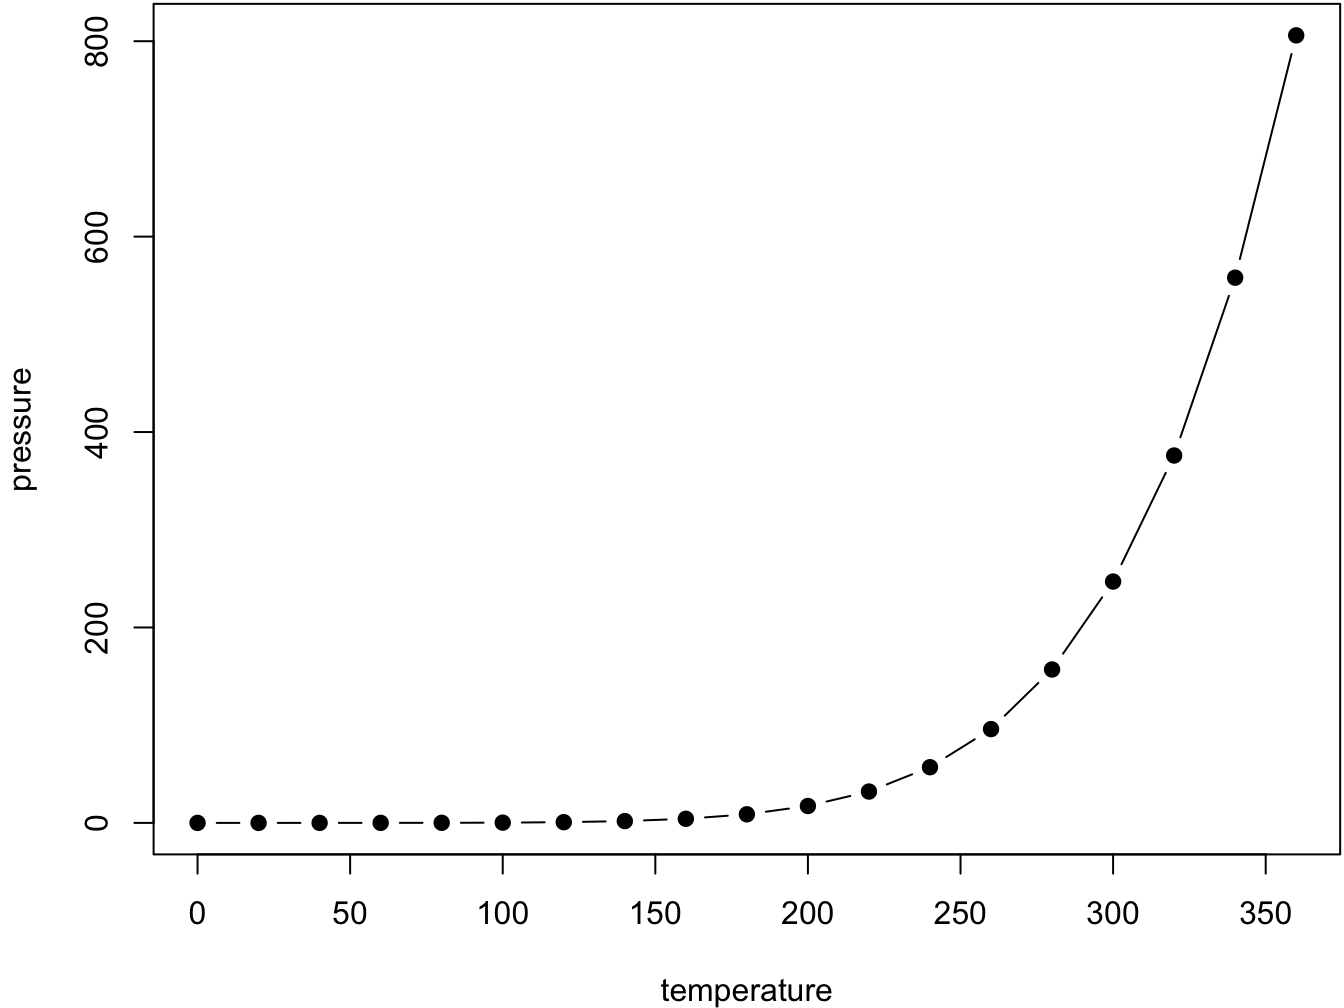
\includegraphics[width=0.8\linewidth]{bookdown-demo_files/figure-latex/nice-fig-1} 

}

\caption{Here is a nice figure!}\label{fig:nice-fig}
\end{figure}

Reference a figure by its code chunk label with the \texttt{fig:}
prefix, e.g., see Figure \ref{fig:nice-fig}. Similarly, you can
reference tables generated from \texttt{knitr::kable()}, e.g., see Table
\ref{tab:nice-tab}.

\begin{Shaded}
\begin{Highlighting}[]
\NormalTok{knitr}\OperatorTok{::}\KeywordTok{kable}\NormalTok{(}
  \KeywordTok{head}\NormalTok{(iris, }\DecValTok{20}\NormalTok{), }\DataTypeTok{caption =} \StringTok{'Here is a nice table!'}\NormalTok{,}
  \DataTypeTok{booktabs =} \OtherTok{TRUE}
\NormalTok{)}
\end{Highlighting}
\end{Shaded}

\begin{table}

\caption{\label{tab:nice-tab}Here is a nice table!}
\centering
\begin{tabular}[t]{rrrrl}
\toprule
Sepal.Length & Sepal.Width & Petal.Length & Petal.Width & Species\\
\midrule
5.1 & 3.5 & 1.4 & 0.2 & setosa\\
4.9 & 3.0 & 1.4 & 0.2 & setosa\\
4.7 & 3.2 & 1.3 & 0.2 & setosa\\
4.6 & 3.1 & 1.5 & 0.2 & setosa\\
5.0 & 3.6 & 1.4 & 0.2 & setosa\\
\addlinespace
5.4 & 3.9 & 1.7 & 0.4 & setosa\\
4.6 & 3.4 & 1.4 & 0.3 & setosa\\
5.0 & 3.4 & 1.5 & 0.2 & setosa\\
4.4 & 2.9 & 1.4 & 0.2 & setosa\\
4.9 & 3.1 & 1.5 & 0.1 & setosa\\
\addlinespace
5.4 & 3.7 & 1.5 & 0.2 & setosa\\
4.8 & 3.4 & 1.6 & 0.2 & setosa\\
4.8 & 3.0 & 1.4 & 0.1 & setosa\\
4.3 & 3.0 & 1.1 & 0.1 & setosa\\
5.8 & 4.0 & 1.2 & 0.2 & setosa\\
\addlinespace
5.7 & 4.4 & 1.5 & 0.4 & setosa\\
5.4 & 3.9 & 1.3 & 0.4 & setosa\\
5.1 & 3.5 & 1.4 & 0.3 & setosa\\
5.7 & 3.8 & 1.7 & 0.3 & setosa\\
5.1 & 3.8 & 1.5 & 0.3 & setosa\\
\bottomrule
\end{tabular}
\end{table}

You can write citations, too. For example, we are using the
\textbf{bookdown} package \citep{R-bookdown} in this sample book, which
was built on top of R Markdown and \textbf{knitr} \citep{xie2015}.

\chapter{Forstmann et al. Dataset}\label{forstmann-et-al.-dataset}

Here is an example dataset. We will use the dataset from
\citet{forstmann2008striatum}.

What packages required? Are they mentioned here? with r code? Version of
R?

First we need to install the psamplers package

\begin{Shaded}
\begin{Highlighting}[]
\KeywordTok{library}\NormalTok{(psamplers)}
\end{Highlighting}
\end{Shaded}

\section{Description of Forstmann
experiment}\label{description-of-forstmann-experiment}

Forstmann et al looked at neural correlates of decision making under
time pressure, with an aim to identify areas of the brain associated
with speed-accuracy tradeoff. Imaging (fMRI) and behavioural data was
collected; however, we'll look at the behavioural data from the
decision-making task only. In terms of modelling the data, Forstmann
expected to find differences in thresholds (direction?) for each of the
three speed-emphasis conditions.

Table \ref{tab:forsthead10} shows the first ten trials from the
Forstmann dataset ( show to get an idea of the data structure?).
Participants \texttt{(n\ =\ 19)} were asked to indicate whether a cloud
of dots in a random-dot kinematogram (RDK) moved to the left or the
right of the screen. The IV was a within-subject, speed-accuracy
manipulation where, before each trial began, pariticipants were
instructed to make their choice accurately \texttt{(condition\ =\ 1)},
with urgency\texttt{(condition\ =\ 3)}or were confronted with a neutral
message \texttt{(condition\ =\ 2)}. Choice and response time data was
collected. Choices were coded as correct \texttt{(correct\ =\ 2)} or
incorrect \texttt{(correct\ =\ \ 1)} and response times \texttt{(rt)}
were recorded in seconds. For more information about the design of the
experiment please see
\href{https://www.pnas.org/content/105/45/17538.short}{the original
paper}.

\begin{table}

\caption{\label{tab:forsthead10}First 10 trials in Forstmann dataset. The `forstmann` dataset is a data frame }
\centering
\begin{tabular}[t]{r|r|r|r}
\hline
subject & rt & correct & condition\\
\hline
1 & 0.4319 & 2 & 1\\
\hline
1 & 0.5015 & 2 & 3\\
\hline
1 & 0.3104 & 2 & 3\\
\hline
1 & 0.4809 & 2 & 1\\
\hline
1 & 0.3415 & 2 & 1\\
\hline
1 & 0.3465 & 2 & 2\\
\hline
1 & 0.3572 & 2 & 2\\
\hline
1 & 0.4042 & 2 & 2\\
\hline
1 & 0.3866 & 2 & 2\\
\hline
1 & 0.3683 & 2 & 1\\
\hline
\end{tabular}
\end{table}

\section{Using the sampler}\label{using-the-sampler}

In this example, we will use the Linear Ballistic Accumulator (LBA)
\citet{brown2008simplest}. The LBA model parameters are: \texttt{b}
threshold parameter (the evidence required to make a response),
\texttt{v} is drift rate or average speed of evidence accumulation,
\texttt{A} is the model's start point and \texttt{t0} is non-decision
time. Do we need to mention \texttt{sv} here?

First, we create a vector of parameter names for the model \texttt{pars}

\begin{Shaded}
\begin{Highlighting}[]
\NormalTok{pars <-}\StringTok{ }\KeywordTok{c}\NormalTok{(}\StringTok{"b1"}\NormalTok{, }\StringTok{"b2"}\NormalTok{, }\StringTok{"b3"}\NormalTok{, }\StringTok{"A"}\NormalTok{, }\StringTok{"v1"}\NormalTok{, }\StringTok{"v2"}\NormalTok{, }\StringTok{"t0"}\NormalTok{)}
\end{Highlighting}
\end{Shaded}

For this dataset, we use 3 threshold parameters (\texttt{b1},
\texttt{b2}, and \texttt{b3}) because we expect threshold to vary as a
function of speed-emphasis instruction. We include two drift rate
parameters: \texttt{v1} for the incorrect accumulator and \texttt{v2}
for the correct accumulator, a start point parameter \texttt{A} and a
non-decision time \texttt{t0} parameter. Note: It is important that the
parameters you list in the \texttt{pars} vector match the names and
number of parameters you include in your log likelihood function. We've
made a decision to set the \texttt{sv} to 1 to satisfy the scaling
properties of the model, as such we haven't included the \texttt{sv}
parameter in the \texttt{pars} vector.

In the new estimations paper pg 6 has an equation with a vector of
individual parameters/random effects - include here?

Next we create a \texttt{priors} object; a list that contains two
components: - Gavin needs to check this priors object stuff *
\texttt{theta\_mu} a vector containing the prior for model parameter
means * \texttt{theta\_sig} the prior covariance matrix for model
parameters.

\begin{Shaded}
\begin{Highlighting}[]
\NormalTok{priors <-}\StringTok{ }\KeywordTok{list}\NormalTok{(}\DataTypeTok{theta_mu =} \KeywordTok{rep}\NormalTok{(}\DecValTok{0}\NormalTok{, }\KeywordTok{length}\NormalTok{(pars)),}
  \DataTypeTok{theta_sig =} \KeywordTok{diag}\NormalTok{(}\KeywordTok{rep}\NormalTok{(}\DecValTok{1}\NormalTok{, }\KeywordTok{length}\NormalTok{(pars)))}
\NormalTok{)}
\end{Highlighting}
\end{Shaded}

The next step is to source your log likelihood function/script. This
must be called before you create the sampler object in the next step.

\begin{Shaded}
\begin{Highlighting}[]
\KeywordTok{source}\NormalTok{(}\DataTypeTok{file =} \StringTok{"yourLogLikelihoodFile.R"}\NormalTok{)}
\end{Highlighting}
\end{Shaded}

We need to supply LBA\_loglike file

Next step is to initialise the \texttt{sampler} object.

\begin{Shaded}
\begin{Highlighting}[]
\NormalTok{sampler <-}\StringTok{ }\KeywordTok{pmwgs}\NormalTok{(}
  \DataTypeTok{data =}\NormalTok{ dataO,}
  \DataTypeTok{pars =}\NormalTok{ pars,}
  \DataTypeTok{prior =}\NormalTok{ priors,}
  \DataTypeTok{ll_func =}\NormalTok{ lba_loglike}
\NormalTok{)}
\end{Highlighting}
\end{Shaded}

The \texttt{pmwgs} function takes a set of arguments listed below and
returns a list containing the required components for performing the
particle metropolis within Gibbs steps.

\begin{itemize}
\tightlist
\item
  \texttt{data\ =} your data (a data frame containing a column for
  participants called `subject')
\item
  \texttt{pars\ =} the model parameters to be used (\texttt{pars} vector
  specified above)
\item
  \texttt{prior\ =} the priors to be used (\texttt{priors} object)
\item
  \texttt{ll\_func\ =} name of log likelihood function you've sourced
  above.
\end{itemize}

You have the option to set model start points. We have specified
sensible start points for the Forstmann dataset. If you chose not to
specify start points, the sampler will randomly sample points from the
prior distribution.

\begin{Shaded}
\begin{Highlighting}[]
\NormalTok{start_points <-}\StringTok{ }\KeywordTok{list}\NormalTok{(}
  \DataTypeTok{mu =} \KeywordTok{c}\NormalTok{(.}\DecValTok{2}\NormalTok{, .}\DecValTok{2}\NormalTok{, .}\DecValTok{2}\NormalTok{, .}\DecValTok{4}\NormalTok{, .}\DecValTok{3}\NormalTok{, }\FloatTok{1.3}\NormalTok{, }\OperatorTok{-}\DecValTok{2}\NormalTok{),}
  \DataTypeTok{sig2 =} \KeywordTok{diag}\NormalTok{(}\KeywordTok{rep}\NormalTok{(.}\DecValTok{01}\NormalTok{, }\KeywordTok{length}\NormalTok{(pars)))}
\NormalTok{)}
\end{Highlighting}
\end{Shaded}

The \texttt{start\_points} object contains two vectors: \texttt{mu} a
vector of start points for the mu of each model parameter and a
\texttt{sig2} vector containing the start points of the covariance
matrix of covariance between model parameters.

Okay - now we are ready to run the sampler.

\begin{Shaded}
\begin{Highlighting}[]
\NormalTok{sampler <-}\StringTok{ }\KeywordTok{init}\NormalTok{(sampler, }\DataTypeTok{theta_mu =}\NormalTok{ start_points}\OperatorTok{$}\NormalTok{mu,}
                \DataTypeTok{theta_sig =}\NormalTok{ start_points}\OperatorTok{$}\NormalTok{sig2)}
\end{Highlighting}
\end{Shaded}

Here we are using the \texttt{init} function to generate initial start
points for the random effects and storing them in \texttt{sampler}
object. First we pass the \texttt{sampler} object from above that
includes our data, parameters, priors and log likelihood function. If we
decided to specify our own start points (as above), we would include the
\texttt{theta\_mu} and \texttt{theta\_sig} arguments.

Now we can run the sampler using the \texttt{run\_stage} function. First
we pass our \texttt{sampler} object that includes the parameters. The
\texttt{stage\ =} argument specifies the sampling stage.
\texttt{iter\ =} is the number of iterations of the sampling stage.
\texttt{particles\ =} is the number of particles generated on each
iteration. It is optional to include the \texttt{iter\ =} and
\texttt{particles\ =} arguments. If these are not included, default
values of 1000 are used. The number of iterations you choose for your
burn in stage is similar to choices made when running deMCMC, however,
this varies depending on the time the model takes to reach the `real'
posterior space.

First we run our burn in stage by setting \texttt{stage\ =} to
\texttt{"burn"}

\begin{Shaded}
\begin{Highlighting}[]
\NormalTok{burned <-}\StringTok{ }\KeywordTok{run_stage}\NormalTok{(sampler, }\DataTypeTok{stage =} \StringTok{"burn"}\NormalTok{, }\DataTypeTok{iter =} \DecValTok{500}\NormalTok{, }\DataTypeTok{particles =} \DecValTok{1000}\NormalTok{)}
\end{Highlighting}
\end{Shaded}

Here we have set iterations to be 500, which may take some time.

\begin{Shaded}
\begin{Highlighting}[]
\NormalTok{adapted <-}\StringTok{ }\KeywordTok{run_stage}\NormalTok{(burned, }\DataTypeTok{stage =} \StringTok{"adapt"}\NormalTok{)}
\end{Highlighting}
\end{Shaded}

Now we run our adaptation stage by setting \texttt{stage\ =\ "adapt"}
Because we have not specified number of iterations or particles, the
sampler will use the default values of 1000 for each of these arguments.
N.B. The sampler will quit adaptation stage after 20 unique values have
been accepted for each subject. This means adaptation may not use all
1000 iterations.

\begin{Shaded}
\begin{Highlighting}[]
\NormalTok{sampled <-}\StringTok{ }\KeywordTok{run_stage}\NormalTok{(adapted, }\DataTypeTok{stage =} \StringTok{"sample"}\NormalTok{, }\DataTypeTok{iter =} \DecValTok{100}\NormalTok{, }\DataTypeTok{particles =} \DecValTok{100}\NormalTok{)}
\end{Highlighting}
\end{Shaded}

At the start of the \texttt{sampled} stage, the sampler object will
create a `proposal' distribution for each subject's random effects using
a conditional multi-variate normal. This proposal distribution is then
used to efficiently generate new particles for each subject which means
we can reduce the number of particles on each iteration whilst still
achieving acceptance rates.

\chapter{The Linear Ballistic
Aclimatiser}\label{the-linear-ballistic-aclimatiser}

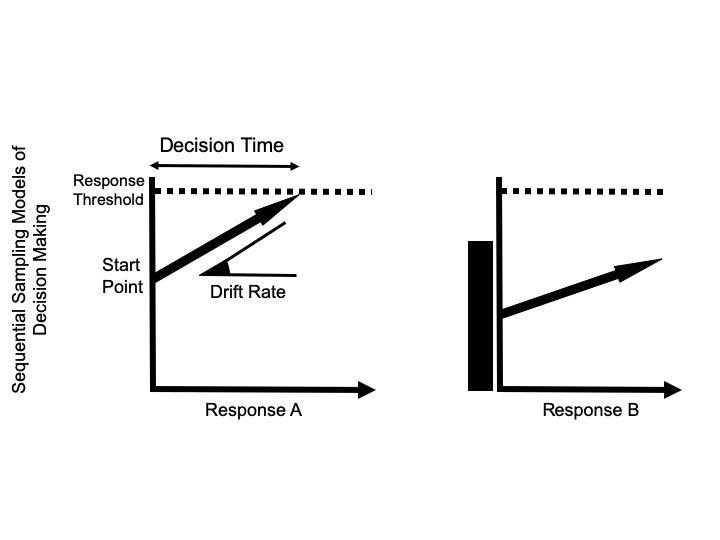
\includegraphics[width=10in]{_images/LBA} The LBA model of
decision-making which explains the trade off between speed and caution.
A basic framework for a simple two choice paradigm is shown. The two
accumulators ``race'' by accumulating evidence for either decision
before reaching the response threshold. The first accumulator to reach
the threshold triggers the associated decision.

\chapter{Applications}\label{applications}

Some \emph{significant} applications are demonstrated in this chapter.

\section{Example one}\label{example-one}

\section{Example two}\label{example-two}

\chapter{Final Words}\label{final-words}

Nice book - dickheads.

\bibliography{book.bib,packages.bib}

\end{document}
